\subsection{インターフェースの設計}
Fortran/C言語インターフェースを開発する上での一つの困難は,FortranやC言語からC++のテンプレート機能を直接利用する手段がないことである.二節で述べた通り,C++のテンプレート機能はFDPSに任意の粒子データ型や粒子間相互作用をサポートさせる上で不可欠なものであった.したがって,Fortran/C言語インターフェースでも任意の粒子データ型や粒子間相互作用をサポートするためには,何らかの方法でこの問題を解決する必要がある.

我々は以下の事柄を組み合わせてこの問題を解決した.(i) C++関数は\texttt{extern "C"}修飾子によってC言語からも呼び出せる事,(ii) FDPSのC++コア部(C++で実装されたFDPSの部分)を操作するC++プログラムの自動生成,(iii) Fortran 2003で導入されたFortranとC言語の相互運用を保証する仕組み.(i)と(iii)によって,\textsl{特定の}粒子データ型向けに作られたFDPSライブラリ(C++コア部を操作する一連のC++関数群のことと定義)をFortranやC言語から利用可能になる.しかしながら,実現したいのは\textsl{任意の}粒子データ型を扱えるFDPSライブラリをFortranやC言語から利用できるようにすることである.これを実現する唯一の方法は,与えられた粒子データ型に応じたFDPSライブラリを生成することである.我々はFDPSの利用者がFortanやC言語のみで,アプリケーションを開発できるようにしたいので,それぞれの言語で粒子を表すデータ構造からFDPSライブラリを生成する必要がある.我々は粒子を表すためのデータ構造として,Fortranでは派生データ型,C言語では構造体を採用した.したがって,我々の解決案は次のようなものである.まず,FDPSの利用者は Fortran 2003の派生データ型 或いは C言語の構造体で粒子を定義する.次に,この粒子データ型に対応するC++クラスを生成する.最後に,このC++クラス向けのFDPSライブラリを生成する.これが(ii)が必要な理由である.これらの生成は我々が用意する\textsc{Python}スクリプトが自動的に行う.

残る問題点は,どのようにしてFortran 或いは C言語で書かれた粒子データ型から対応するC++クラスを生成するのかということである.適切な生成には,以下の情報が必要となる.
\begin{itemize}
\item データ型が粒子を表すものであること.
\item データ型のどのメンバ変数がFDPSが必要とする物理量に対応するか.FDPSは粒子の位置等,特定の物理量を必要とする.C++からFDPSを利用する場合,利用者に位置を返すメンバ関数等,いくつかのメンバ関数を定義してもらうことでこの問題を解決する設計となっていた.しかしながら,Fortranの派生データ型やC言語の構造体はメンバ関数は持てない.
\end{itemize}
我々は独自の指示文を導入してこの問題を解決した.指示文は特定のフォーマットのコメント文で,自動生成を行う\textsc{Python}スクリプトに必要な情報を渡すために使用される.具体的には,例えばFortranの場合,派生データ型名の隣にコメント文\texttt{!\$fdps FP}を記述すると,スクリプトは,この派生データ型がFullParticle型であると解釈する.ここで,FullParticle型は粒子のすべての情報を持つデータ型のことである.同様に,メンバ変数名の隣にコメント文\texttt{!\$fdps position}を記述すると,このメンバ変数は粒子の位置を表すとスクリプトは解釈する.このような指示文を用いることで,スクリプトは必要なC++クラスを生成することが可能となる.

以上がFortran/C言語インターフェースの設計である.図\ref{fig:if_design}は,インターフェースの仕組みを模式的に表したものである.まずユーザは粒子をFortranの派生データ型 或いは C言語の構造体で定義する.このとき,指示文を使って必要な情報も記述する(ステップ\ding{192}).自動生成スクリプトは,ユーザが書いたソースコードの中から指示文を手がかりに粒子を表す派生データ型 ないしは 構造体を自動的にすべて見つけ,対応するC++クラスを(複数)生成する(ステップ\ding{193}).同時に,これらC++クラス向けのFDPSライブラリを生成する(ステップ\ding{194}).これはC++から利用可能なFDPSのAPIとほぼ同じものを提供するC++関数群から構成される.スクリプトはこのC++関数群のC言語インターフェースも生成する(ステップ\ding{195}).これがFDPSのC言語インターフェースと呼んでいるものである.Fortranから使用可能にするためのFortranモジュールも生成される(ステップ\ding{196}).このモジュールはFortran用のインターフェースを提供する.ユーザはこれらのインターフェースで提供されるAPIを使用して,アプリケーションを開発する(ステップ\ding{197}, \ding{197}').
\begin{figure}
\centering
\includegraphics[width=8cm]{./fig/if_design.eps}
\caption{Fortran/C言語インターフェースの仕組み}
\label{fig:if_design}
\end{figure}

\subsection{インターフェースの利用例}
本節ではC言語インターフェースの利用例を簡単に説明する.前節で述べた通り,ユーザはまずC言語の構造体と指示文を用いて粒子を定義する必要がある.そこで,粒子を定義したC言語ソースファイルの例を図\ref{fig:src_fp_in_c}に示す.
\begin{figure}
\centering
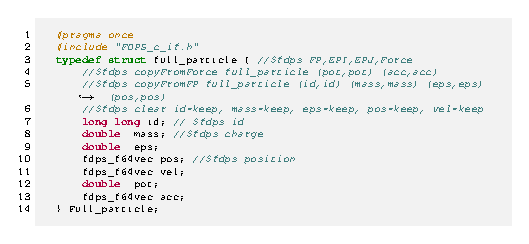
\includegraphics[width=8cm]{./fig/src_fp_in_c.eps}
\caption{C言語での粒子の実装例}
\label{fig:src_fp_in_c}
\end{figure}
上から順に説明していく.まず,ファイル冒頭でヘッダーファイル\texttt{FDPS\_c\_if.h}がインクルードされている.このヘッダーファイルにはFDPSのC言語用APIのプロトタイプ宣言やFDPSから提供されるデータ型が記述されており,これらを使用する場合には必ずインクルードする必要がある.

次に構造体タグ名の右隣に以下のコメント文がある.
\begin{lstlisting}
//$fdps FP,EPI,EPJ,Force
\end{lstlisting}
これはこの構造体が粒子であることを示す指示文である.文字列\texttt{//\$fdps}で始まるコメント文はすべて自動生成スクリプトに指示文として解釈される.文字列\texttt{//\$fdps}の右側には粒子の種別を表すキーワードが続いる.\texttt{FP}はFullParticle型,\texttt{EPI}はEssentialParticleI型,\texttt{EPJ}はEssentialParticleJ型,\texttt{Force}はForce型であることを示すキーワードである.複数のキーワードが指定された場合,それらを同時に兼ねることを示す.FullParticle型以外のデータ型の定義についてはFDPSの仕様書を参照されたい.

メンバ変数宣言部の前の部分(3-6行目)に3つの指示文がある.これらはFDPS内部でのデータ処理の仕方を指示するための指示文である.こちらも詳細については,仕様書を参照されたい.

メンバ変数宣言部に注目すると,いくつかのメンバ変数の右隣に指示文がある.文字列\texttt{//\$fdps}に続く文字列はどの物理量に対応しているかを示すキーワードであり,\texttt{id}は粒子ID,\texttt{charge}は電荷(質量),\texttt{position}は位置を表す.

次にメイン関数の実装例を図\ref{fig:src_main_in_c}に示す.紙面の都合上,ヘッダーファイルのインクルード等の部分は省いた.ここで使用されている関数の内,関数名が\texttt{fdps\_}で始まるものはすべてC言語用のAPIである.図\ref{code:main}と比較してみると,使用しているAPIは異なるが,全体的な構造はC++で実装する場合と似た構造となる.すなわち,はじめにFDPSを初期化するためのAPIを呼び出す(API \texttt{fdps\_initialize}).次に,\texttt{DomainInfo}, \texttt{ParticleSystem}, \texttt{TreeForForce}オブジェクトを生成・初期化する(API \texttt{fdps\_create\_*}, \texttt{fdps\_init\_*} [\texttt{*}は正規表現]).そして,これらを使って,領域分割(API \texttt{fdps\_decompose\_domain\_all}),粒子交換(API \texttt{fdps\_exchange\_particle}),そして相互作用計算(API \texttt{fdps\_calc\_force\_all\_and\_write\_back})を行う,という構造となっている.


\begin{figure}
\centering
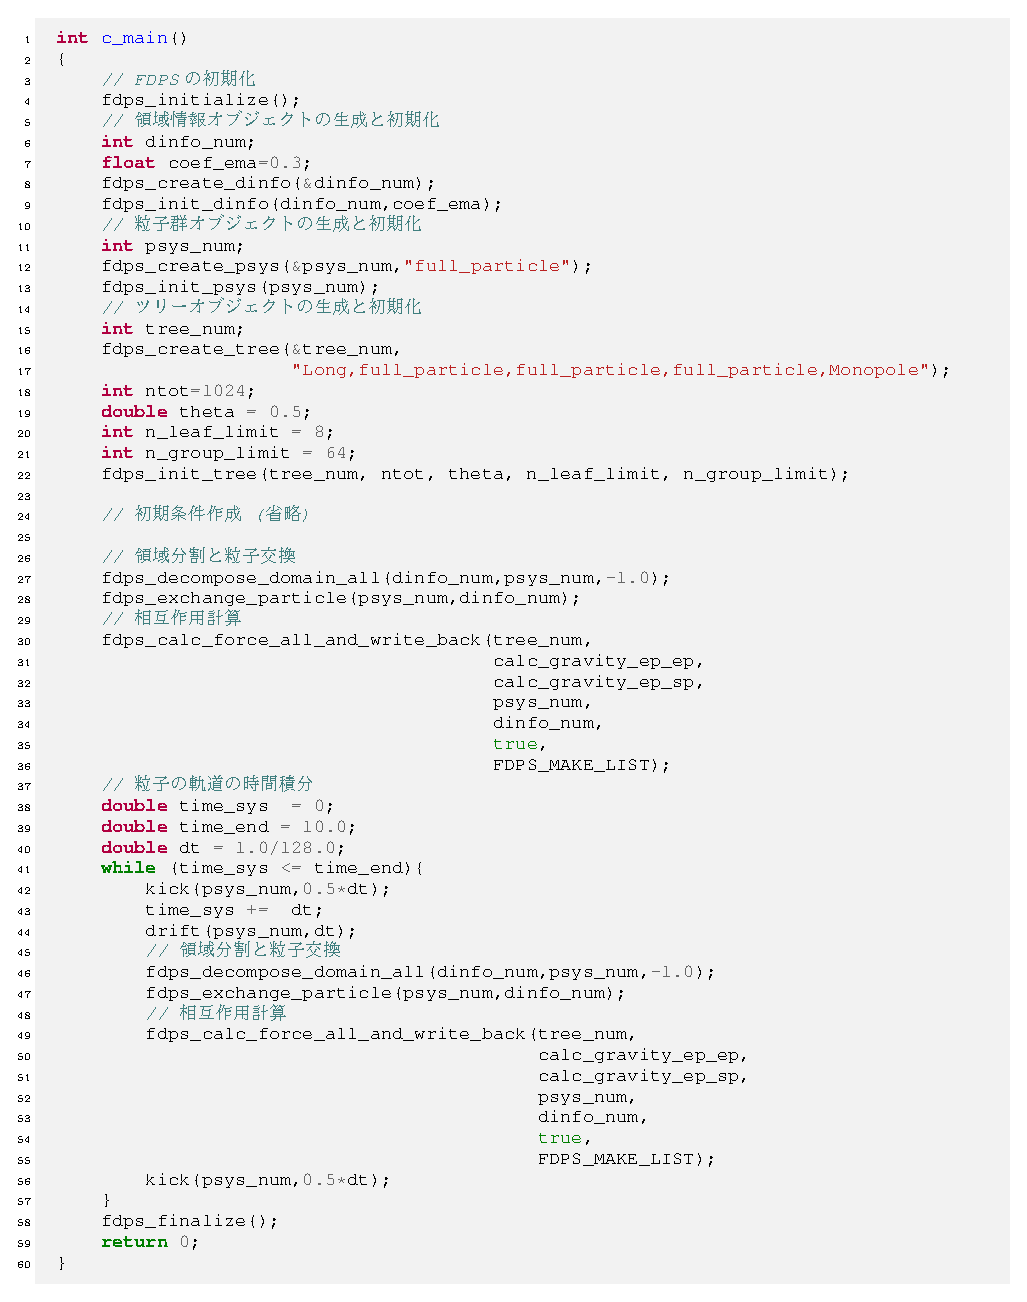
\includegraphics[width=8cm]{./fig/src_main_in_c.eps}
\caption{C言語でのメイン関数の実装例.関数\texttt{drift}, \texttt{kick}は,それぞれ粒子の位置と速度を時間積分する関数である.また,関数\texttt{calc\_gravity\_ep\_ep}, \texttt{calc\_gravity\_ep\_sp}はそれぞれ粒子間相互作用,粒子-超粒子間相互作用を計算する関数である.}
\label{fig:src_main_in_c}
\end{figure}


以上,C言語インターフェースの利用例についての簡単な説明を行った.Fortranインターフェースを用いる場合でも,メイン関数の構造はほぼ同じ構造となる.Fortranインターフェースを使った例に関しては,FDPSに付属するドキュメントや\cite{2018PASJ...70...70N}を参照されたい.
